\documentclass{ctexart}
\title{\heiti \zihao{2} 希腊值的推导与实现}
\author{\heiti \zihao{5}杨宸宇\\\heiti \zihao{5}2016301550186}
\date{}
\pagestyle {plain}
\usepackage{amsmath}
\usepackage{listings}
\usepackage{color}
\usepackage{graphicx}

\definecolor{dkgreen}{rgb}{0,0.6,0}
\definecolor{gray}{rgb}{0.5,0.5,0.5}
\definecolor{mauve}{rgb}{0.58,0,0.82}

\lstset{frame=tb,
  language=Python,
  aboveskip=3mm,
  belowskip=3mm,
  showstringspaces=false,
  columns=flexible,
  basicstyle={\small\ttfamily},
  numbers=none,
  numberstyle=\tiny\color{gray},
  keywordstyle=\color{blue},
  commentstyle=\color{dkgreen},
  stringstyle=\color{mauve},
  breaklines=true,
  breakatwhitespace=true,
  tabsize=3
}
\begin{document}
    \maketitle
    
    \noindent 我们已知看涨期权定价公式为:
    \begin{align}
        C=SN(d_1)-Ke^{-r(T-t)}N(d_2)
    \end{align}
    其中:
    \begin{align}
        d_1 & = \frac{\ln{(S/K)}+(r+\sigma^{2}/2)(T-t)}{\sigma\sqrt{(T-t)}}\\
        d_2 & = \frac{\ln{(S/K)}+(r-\sigma^{2}/2)(T-t)}{\sigma\sqrt{(T-t)}}\\
        d_2 & = d_1 - \sigma \sqrt{(T-t)}\label{d12}\\
        N(\alpha) & = \int_{-\infty}^\alpha \frac{1}{\sqrt{2\pi}}e^{-\frac{x^{2}}{2}}dx
    \end{align}
    然后以此为基础对5个希腊值进行推导


    \section{Delta}
    \noindent Delta是C对S的一阶偏导数,于是我们有如下证明:
    \begin{align}
        \frac{\partial C}{\partial S} & = N(d_1)+S*\frac{\partial N(d_1)}{\partial S}-Ke^{r(T-t)}*\frac{\partial N(d_2)}{S}\\
        & = N(d_1)+S*\frac{\partial N(d_1)}{\partial S}-Ke^{r(T-t)}*\frac{\partial N(d_2)}{S}
    \end{align}
    我们可以得到:
    \begin{align}
        \frac{\partial N(d_1)}{\partial S} & = \frac{1}{\sqrt{2\pi}}e^{-\frac{d_1^2}{2}}*d'_1\\
        \frac{\partial N(d_2)}{\partial S} & = \frac{1}{\sqrt{2\pi}}e^{-\frac{d_2^2}{2}}*d'_2\\
        \frac{\partial d_1}{\partial S}  & =  \frac{1}{\sigma\sqrt{(T-t)}}*\frac{K}{S}*\frac{1}{K}\notag \\
             & =  \frac{1}{\sigma S \sqrt{(T-t)}}\\
        \frac{\partial d_2}{\partial S}  & =  \frac{1}{\sigma S \sqrt{(T-t)}}
    \end{align}
    因此,原始式子转换成:
    \begin{align}
        \frac{\partial C}{\partial S} & = N(d_1)+\frac{1}{\sigma \sqrt{2\pi (T-t)}}e^{-\frac{d^2_1}{2}}-\frac{Ke^{-r(T-t)}}{\sigma S \sqrt{2\pi (T-t)}}e^{-\frac{d^2_2}{2}} \label{delta}
    \end{align}
    计算$d_1^2$和$d_2^2$,我们得到:
    \begin{align}
        d_1^2 & = \frac{\ln^2{(S/K)}+(r+\sigma ^2 /2)^2 (T-t)^2 + 2\ln{(S/K)}(r+\sigma ^2/2)(T-t)}{\sigma^2 (T-t)}\\
        d_2^2 & = \frac{\ln^2{(S/K)}+(r-\sigma ^2 /2)^2 (T-t)^2 + 2\ln{(S/K)}(r-\sigma ^2/2)(T-t)}{\sigma^2 (T-t)}
    \end{align}

    \noindent 发现其中有公共因子,提取出来,令:
    \begin{align}
        A  = \frac{1}{\sigma \sqrt{2\pi (T-t)}} e^{-\frac{\ln^2(S/K)+(r^2+\sigma^4/4)(T-t)^2}{2\sigma ^2 (T-t)}}
    \end{align}
    \noindent 于是,我们可以见 \eqref{delta}中的后两项进行化简:
    \begin{align}
        B = \frac{1}{\sigma \sqrt{2\pi (T-t)}}e^{-\frac{d^2_1}{2}}-\frac{Ke^{-r(T-t)}}{\sigma S \sqrt{2\pi (T-t)}}e^{-\frac{d^2_2}{2}}
    \end{align}
    \begin{align}
        B & = A*(e^{(\frac{-r\sigma ^2 (T - t)+2\ln{(S/K)}+(r+\sigma ^2/2)}{\sigma ^2})} - \frac{Ke^r(T-t)}{S}e^{(\frac{r\sigma ^2 (T - t)+2\ln{(S/K)}-(r+\sigma ^2/2)}{\sigma ^2})})\notag \\
        & = A*(e^{-\frac{r(T-t)}{2}}*e^{-\frac{\ln(S/K)}{2}}-\frac{Ke^{-r(T-t)}}{S}e^{\frac{r(T-t)}{2}}*e^{\frac{\ln(S/K)}{2}})\notag \\
        & = A*(e^{-\frac{r(T-t)}{2}}*e^{-\frac{\ln(S/K)}{2}}-\left(S/K\right)^{-1}*e^{\frac{-r(T-t)}{2}}*e^{\frac{\ln(S/K)}{2}})\notag \\
        & = A*(e^{-\frac{r(T-t)}{2}}*e^{-\frac{\ln(S/K)}{2}}-e^{-\frac{r(T-t)}{2}}*e^{-\frac{\ln(S/K)}{2}})\notag \\
        & = 0
    \end{align}
    \noindent 因此 我们最终得到:
    \begin{align}
        \boldsymbol{\Delta} & = N(d_1)
    \end{align}
    
    \noindent 同时\eqref{delta}后两项相等,我们得到一个结论,之后会用到:
    \begin{align}
        SN'(d_1) & = Ke^{-r(T-t)}N'(d_2)\label{Equel}
    \end{align}
    其中:
    \begin{align}
        N'(d_1) & = \frac{1}{\sqrt{2\pi}}e^{-\frac{d^{2}_1}{2}}\label{N'(d1)}\\
        N'(d_2) & = \frac{1}{\sqrt{2\pi}}e^{-\frac{d^{2}_2}{2}}
    \end{align}\\

    


    \section{Gamma}   
    \noindent Gamma是C对S的二阶导数,即Delta对S的一阶导数,我们有如下证明:
    \begin{align}
         \frac{\partial \delta}{\partial S}  & = \frac{\partial N(d_1)}{\partial S}\notag \\
        & = \frac{1}{\sqrt{2\pi}}e^{-\frac{d^2_1}{2}}*\frac{\partial d_1}{\partial S}\notag \\
        & = \frac{1}{\sqrt{2\pi}}e^{-\frac{d^2_1}{2}}*\frac{1}{\sigma S \sqrt{T-t}}\notag \\
        & = \frac{1}{\sqrt{2\pi (T-t)}\sigma S}e^{-\frac{d^2_1}{2}}
    \end{align}
    所以我们得到:
    \begin{align}
        \boldsymbol{\Gamma} & = \frac{1}{\sigma S\sqrt{2\pi (T-t)}}e^{-\frac{d^2_1}{2}}
    \end{align}
    也可以表示为:
    \begin{align}
        \boldsymbol{\Gamma} & = \frac{N'(d_1)}{S\sigma\sqrt{T-t}}
    \end{align}\\
    
    \section{Theta}
    \noindent Theta是C对t的一阶导数,我们有如下证明:
    \begin{align}
        \frac{\partial C}{\partial t} & = N'(d_1)-Ke^{-r(T-t)}rN(d_2)-Ke^{-r(T-t)}N'(d_2)\frac{\partial d_2}{\partial t}\label{original vega}
    \end{align}
    我们根据 \eqref{Equel},可以对\eqref{original vega}进行化简:
    \begin{align}
        \frac{\partial C}{\partial t} & = -rKe^{-r(T-t)}N(d_2)+SN'(d_1)\left(\frac{\partial d_1}{\partial t}-\frac{\partial d_2}{\partial t}\right)
    \end{align}
    根据$d_1$和$d_2$的等价关系\eqref{d12}可以知道:
    \begin{align}
        d_1-d_2 & = \sigma\sqrt{T-t}\\
        \frac{\partial d_1}{\partial t}-\frac{\partial d_2}{\partial t} & =\frac{\partial (\sigma \sqrt{T-t})}{\partial t}\notag\notag \\
        & = -\frac{\sigma}{2\sqrt{T-t}}
    \end{align}
    所以我们最终得到:
    \begin{align}
        \frac{\partial C}{\partial t} & = -rKe^{-r(T-t)}N(d_2) -SN'(d_1)\frac{\sigma}{2\sqrt{T-t}}\\
        \boldsymbol{\Theta} & = -rKe^{-r(T-t)}N(d_2) -SN'(d_1)\frac{\sigma}{2\sqrt{T-t}}
    \end{align}\\
    
    
    \section{Vega}
    \noindent Vega是C对$\sigma$的一阶导数,我们有如下证明:
    \begin{align}
        \frac{\partial C}{\partial \sigma} & = SD'(d_1)\frac{\partial d_1}{\partial \sigma} - Ke^{-r(T-t)}N(d_2)\frac{\partial d_2}{\partial \sigma}
    \end{align}
    同样根据\eqref{d12}和\eqref{Equel}:
    \begin{align}
        \frac{\partial C}{\partial \sigma} & = SN'(d_1)(\frac{\partial d_1}{\partial t}-\frac{\partial d_2}{\partial t})
    \end{align}
    \begin{align}
        \frac{\partial d_1}{\partial t}-\frac{\partial d_2}{\partial t} & = \sqrt{T-t}
    \end{align}
    所以我们最终计算出:
    \begin{align}
        \frac{\partial C}{\partial \sigma} & = SN'(d_1)\sqrt{T-t}\\
        \boldsymbol{V} & = SN'(d_1)\sqrt{T-t}
    \end{align}\\

    
    
    \section{Rho}
    \noindent Rho是C对r的一阶导数,我们有如下证明:
    \begin{align}
        \frac{\partial C}{\partial r} & = SN'(d_1)\frac{\partial d_1}{\partial r}+Ke^{-r(T-t)}(T-t)N(d_2)-Ke^{-r(T-t)}N'(d_2)\frac{\partial d_2}{\partial r}
    \end{align}
    根据等价关系\eqref{d12}和\eqref{Equel}:
    \begin{align}
        SN'(d_1)\frac{\partial d_1}{\partial r} - Ke^{-r(T-t)}N'(d_2)\frac{\partial d_2}{\partial r} &= SN'(d_1)(\frac{\partial d_1}{\partial r}-\frac{\partial d_2}{\partial r})\notag \\
        & = SN'(d_1) * 0\notag \\
        & = 0
    \end{align}
    所以,我们最终得到:
    \begin{align}
        \frac{\partial C}{\partial r} & = (T-t)Ke^{-r(T-t)}N(d_2)\\
        \boldsymbol{\rho} & = (T-t)Ke^{-r(T-t)}N(d_2)
    \end{align}
    \newpage
    \section {Python代码实现}
    \begin{lstlisting}
        # -*-coding:utf-8-*-

        # 主题: 第二次金融工程学实验作业
        # 作者: 杨宸宇
        # 学号: 2016301550186
        # 日期: 11\28\2018

        # 调用所需要的库
        import numpy as np
        import pandas as pd
        import matplotlib.pyplot as plt
        import seaborn as sns
        from math import log, sqrt, exp, pi
        from scipy import stats


        class Greek(object):

            def __init__(self, S0, K, T, r, sigma):
                '''

                :param S0: 标的价格
                :param K: 期权的执行价格
                :param T: 时间
                :param r: 无风险利率
                :param sigma: 波动率

                '''
                self.S0 = S0
                self.K = K
                self.T = T
                self.r = r
                self.sigma = sigma
                self.d1 = (log(self.S0 / self.K) + (self.r + 0.5 * self.sigma ** 2) * self.T) / (self.sigma * sqrt(self.T))
                self.d2 = (log(self.S0 / self.K) + (self.r - 0.5 * self.sigma ** 2) * self.T) / (self.sigma * sqrt(self.T))

            def bs_call_value(self):
                value = (self.S0 * stats.norm.cdf(self.d1, 0., 1.)) \
                        - self.K * exp(-self.r * self.T) * stats.norm.cdf(self.d2, 0., 1.)
                return value

            def delta(self):
                value = stats.norm.cdf(self.d1, 0., 1.)
                return value

            def gamma(self):
                value = 1 / (sqrt(2 * pi * self.T) * self.sigma * self.S0) * exp(-self.d1 ** 2 / 2)
                return value

            def theta(self):
                value = -self.r * self.K * exp(-self.r * self.T) * stats.norm.cdf(self.d2, 0., 1.) \
                        - (self.S0 * 1 / sqrt(2 * pi) * exp(-self.d1 ** 2 / 2) * self.sigma) / (2 * sqrt(self.T))
                return value

            def vega(self):
                value = self.S0 * sqrt(self.T) * 1 / sqrt(2 * pi) * exp(-self.d1 ** 2 / 2)
                return value

            def rho(self):
                value = self.T * self.K * exp(-self.r * self.T) * stats.norm.cdf(self.d2, 0., 1.)
                return value


        # 实验函数结果------------------------------------------
        greek = Greek(49, 50, 0.3846, 0.05, 0.2)
        print("The Delta is %f\nThe Gamma is %f\nThe Theta is %f\nThe Vega is %f\nThe Rho is %f" % (
        greek.delta(), greek.gamma(), greek.theta(), greek.vega(), greek.rho()))

        # 生成各个希腊值的曲线
        # Delta
        data = pd.DataFrame()
        data['S'] = np.linspace(35, 65, 1000)
        data['Delta'] = np.nan
        for i in range(len(data)):
            data.iloc[i, 1] = Greek(data.iloc[i, 0], 50, 0.3846, 0.05, 0.2).delta()
        sns.set()
        p = sns.lineplot(x='S', y='Delta', data=data, color='blue', linewidth=2.5)
        p.set_title('Delta Plot')
        plt.show()

        # Gamma
        data = pd.DataFrame()
        data['S'] = np.linspace(25, 65, 1000)
        data['Gamma'] = np.nan
        for i in range(len(data)):
            data.iloc[i, 1] = Greek(data.iloc[i, 0], 50, 0.3846, 0.05, 0.2).gamma()
        sns.set()
        p = sns.lineplot(x='S', y='Gamma', data=data, color='blue', linewidth=2.5)
        p.set_title('Gamma Plot')
        plt.show()

        # Theta
        data = pd.DataFrame()
        data['S'] = np.linspace(35, 100, 1000)
        data['Theta'] = np.nan
        for i in range(len(data)):
            data.iloc[i, 1] = Greek(data.iloc[i, 0], 50, 2, 0.05, 0.25).theta()
        sns.set()
        p = sns.lineplot(x='S', y='Theta', data=data, color='blue', linewidth=2.5)
        p.set_title('Theta Plot')
        plt.show()

        # Vega
        data = pd.DataFrame()
        data['S'] = np.linspace(30, 65, 1000)
        data['Vega'] = np.nan
        for i in range(len(data)):
            data.iloc[i, 1] = Greek(data.iloc[i, 0], 50, 0.3846, 0, 0.2).vega()
        sns.set()
            p = sns.lineplot(x='S', y='Vega', data=data, color='blue', linewidth=2.5)
        p.set_title('Vega Plot')
        plt.show()

        # Rho
        data = pd.DataFrame()
        data['S'] = np.linspace(35, 65, 1000)
        data['Rho'] = np.nan
        for i in range(len(data)):
            data.iloc[i, 1] = Greek(data.iloc[i, 0], 50, 0.3846, 0.05, 0.2).rho()
        sns.set()
        p = sns.lineplot(x='S', y='Rho', data=data, color='blue', linewidth=2.5)
        p.set_title('Rho Plot')
        plt.show()

    \end{lstlisting} 

    \heiti \zihao{5}各希腊值和标的资产价格变动关系见后页:
    \newpage
    
    \begin{figure}[ht]

        \centering
        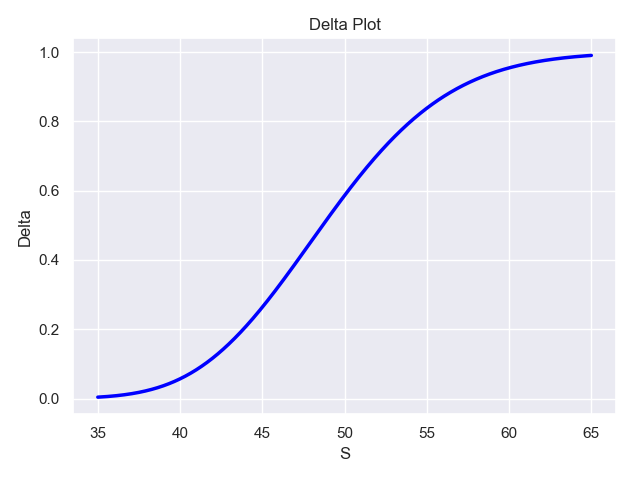
\includegraphics[scale = 0.6]{Delta.JPEG}
        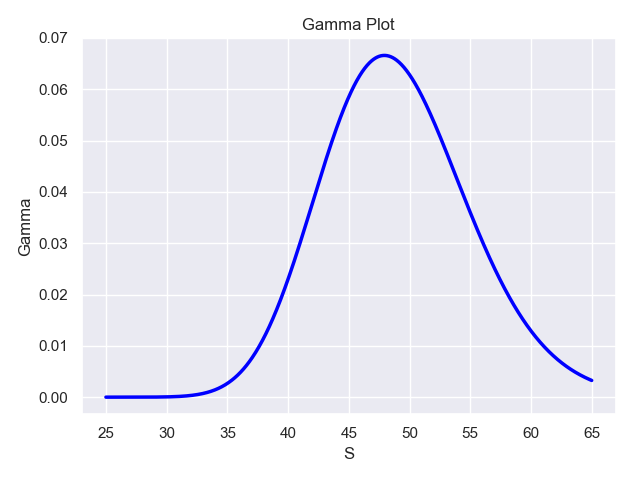
\includegraphics[scale = 0.6]{Gamma.JPEG}
        
    \end{figure}
    \begin{figure}[ht]

        \centering
        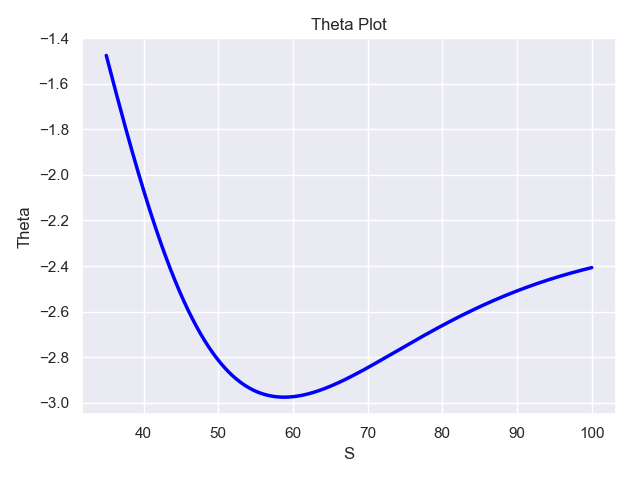
\includegraphics[scale = 0.6]{Theta.JPEG}
        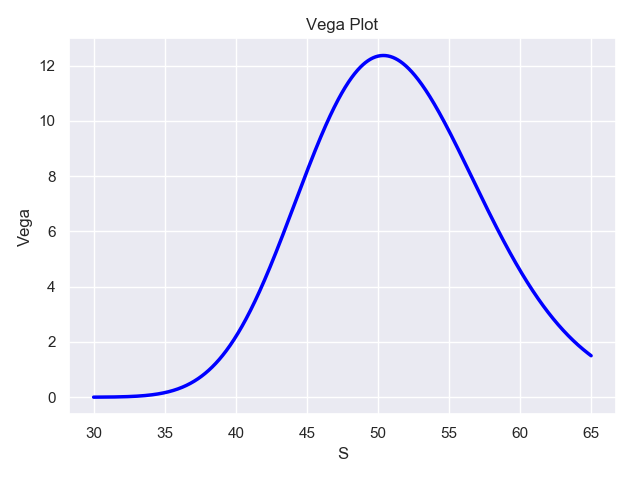
\includegraphics[scale = 0.6]{Vega.JPEG}
        
    \end{figure}
    \begin{figure}

        \centering
        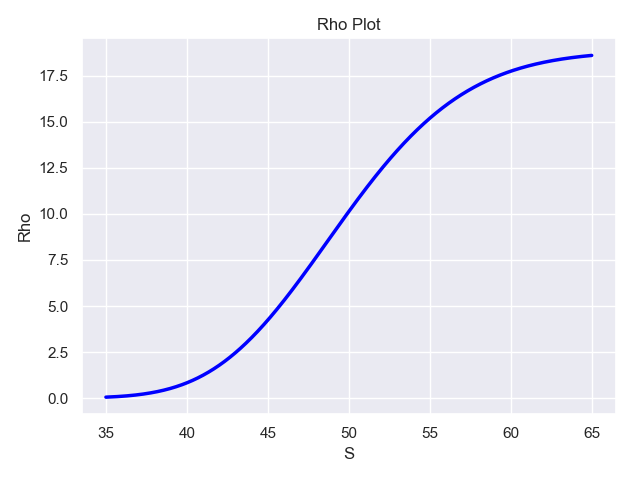
\includegraphics[scale = 0.6]{Rho.JPEG}
        
    \end{figure}


\end{document}